\section{Pronosticando Valores con Regresión}
La regresión lineal es el punto de entrada más sencillo de entender y aplicar en la ciencia de datos. Parte de esto se debe a que la regresión lineal es aplicable en muchos casos a una gran gama de problemas de predicción en los cuales el científico de datos cuenta con una base de datos o juego de datos lo suficientemente grande y accesible para entrenar un modelo. La segunda razón es que un modelo bien entrenado de regresión lineal por lo general nos da una respuesta con cierto grado de precisión que da por cerrado el caso. 

El concepto en sí es relativamente sencillo de abstraer y explicar. En una visualización de datos donde un valor $y$ se corresponde con alguna relación del valor $x$, para cada $x$ y $y$, es posible trazar una línea que en cierta forma sea representativa del valor de predicción de $y$ para cada $x$. Esta línea puede no ser perfecta, o puede dejar muchos puntos sin una relación válida (a menos en el papel de gráfico) pero nos da una idea aproximada de la tendencia y evolución de los datos. \\

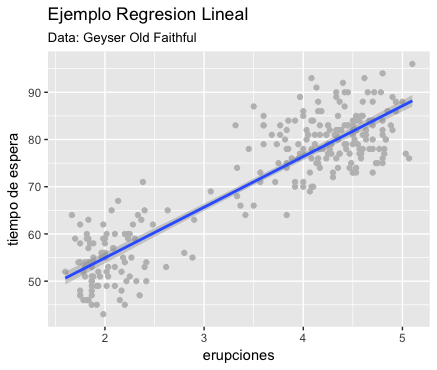
\includegraphics[width = 4 in]{ejemRegresionLineal.png}\\

Zumel y Mount describen la regresión lineal como el más común de los métodos de aprendizaje automatizado \cite{zumelMount}. Para los autores hay una probabilidad muy grande que el método funcione bien con el problema, y si no, es muy fácil verificar cual otro método probar como segunda opción. Para Daroczi, el énfasis está en los modelos de regresión multivariable (una extensión de la regresión lineal simple de un solo predictor y resultado) que construyen el camino para la predicción de fenómenos complejos en la naturaleza y negocios (Daróczi, G., 2015). Por su parte, Harrington resume los beneficios de la regresión lineal (Harrington, P., 2012) por la facilidad de interpretar los resultados y lo frugal en el uso de ciclos de computación (aunque puede ser menos útil si el fenómeno no es perfectamente lineal).

\subsection{Definición de Regresión Lineal}
Downey describe la regresión lineal como aquella que está basada en modelos de funciones lineales \cite{thinkStats}. Para Mann y Lacke la regresión lineal es aquella que se da como una función lineal entre dos variables, y la cual se puede dibujar en el plano cartesiano como una recta \cite{intoStats7}. Yau por su lado, define la regresión lineal simple como el modelo que describe la relación entre dos variables, $x$ y $y$, expresada por la ecuación de regresión lineal, donde $\alpha$ y $\beta$ son parámetros y $\epsilon$ es el término de error \cite{yau}.

La fórmula a la que hacemos referencia en la definición de Yau, y la que utilizan los otros autores, es la siguiente:

\[Y_{i} = \beta_{0} + \beta_{1}X_{i} + \epsilon_{i}\]



\subsection{Regresión Multi-Variable}
Para Downey (Downey, 2015), la regresión múltiple es aquella en la cual se utilizan múltiples variables independientes, pero una sola variable dependiente. 

El Dr. Tattar de la Universidad de Bangalore define que el modelo de regresión línea simple no es realista ni aplicable al mundo practico (Tattar, 2013). Para aplicaciones más reales, es casi obligatorio el uso de modelos de regresión múltiple, en los cuales varias variables independientes se conjugan como parámetros de regresión. 

La regresión multivariable no es un tema mayormente complicado en teoría cómo lo es en llevar a la práctica. No todos los ejemplos de regresiones multivariables nos van a llevar a funciones lineales, sino que estamos tocando el limite entre regresión lineal y métodos de regresión general con funciones no lineales que pueden necesitar de transformaciones matemáticas para obtener un modelo apropiado \cite{daroczi}. Aquí también se explica la selección de un modelo con múltiples variables independientes y cuales conviene seleccionar \cite{viswanathan}.

La mayor parte de la teoría de esta sección sigue el desarrollo de la fórmula:

\[Y_{i} = \beta_{0} + \beta_{1}X_{1} + \beta_{2}X_{2} + \cdots + \epsilon_{i}\]

\subsection{Presunción del Modelo}
Hay cinco factores que deben darse en un modelo cuya presunción es que su muestra sigue una distribución normal. En esta sección revisamos cada uno de esos cinco factores \cite{daroczi}.

\subsection{Calce de los Datos}
Llegar a un modelo de regresión lineal no significa llegar a una solución optima, ni mucho menos. Los datos pueden calzar de forma muy elástica dentro del modelo, por lo que debemos recurrir a los coeficientes de correlación y determinación para verificar si el modelo tiene algún poder predictivo de uso científico

\subsubsection{R - Coeficiente de Correlación de Pearson}
El coeficiente de correlación de Pearson mide la relación lineal entre dos variables aleatorias cuantitativas. La correlación de Pearson es independiente de la escala de medida de las variables, lo que permite tener comparaciones mucho más objetivas independiente del fenómeno estudiado.

De manera menos formal, podemos definir el coeficiente de correlación de Pearson como un índice que puede utilizarse para medir el grado de relación de dos variables siempre y cuando ambas sean cuantitativas.

\[R = \frac{\Sigma(x_i - \bar{x})(y_i - \bar{y})}{\sqrt{\Sigma(x_i - \bar{x})^2\Sigma(y_i - \bar{y})^2}}\]

\subsubsection{R2 - Coeficiente de Determinación}
El coeficiente de determinación - denominado \(R^{2}\) - es un estadístico usado en el contexto de un modelo estadístico cuyo principal propósito es predecir resultados futuros o probar una hipótesis. El coeficiente determina la calidad del modelo para replicar los resultados, y la proporción de variación de los resultados que puede explicarse por el modelo. 

En el caso de regresión lineal, la formula del coeficiente de determinación sigue la siguiente forma:

\[R^{2} = \frac{\sigma^{2}_{XY}}{\sigma^{2}_{X}\sigma^{2}_{Y}}\]

\subsubsection{Valor de p}

\subsection{Seleccionando Variables de Predicción}
Un modelo de regresión de múltiple variables independientes puede tener una solución parsimoniosa sin necesidad de incluir todos sus términos. Esto es verdad cuando la cantidad de variables independientes utilizadas en el análisis 
